\subsection{Skalarum}
En Detektor skal være robust overfor små geometriske og fotometriske deformationer samt støj. Geometriske forskelle kan omfatte rotation, skalering og ændring af perspektiv.  Fotometriske forskelle kan omfatte ændringer i belysning (f.eks. ved delvist overskyet vejr) eller forskelle i refleksion mod de to drone-positioner hvorfra billederne er optaget. En god detektor skal være invariant over for sådanne forskelle. Der er bred enighed om nødvendigheden for skalainvarians hos deteketorer \cite{koen} \cite{blob} \cite{lindenscale}. Dette afsnit beskriver, hvordan en sådan invarians kan opnås. \\ \\
Objekter i virkeligheden, såvel som  af-billedet, optræder kun som meningsfulde enheder over et specifikt skalainterval. Et træ vil indenfor centimeters eller nanometers afstand optræde som blade eller molekyler og indenfor meters afstand som et træ. 
%Koenderink \cite{koen} definere et objekts skalainterval som værende afgrænset af to skalaer, hvor objektet er def: den inderste og den yderste skala, f.eks. vil en trætop have en indre skala på ca. 10 cm og en ydre skala på ca. 10 m. %Da billedet indeholder en ukendt scene, 
Det vides ikke hvilket skalainterval, der er meningsfuldt, for et givent objekt i en scene. 
%Den inderste skala af billedet vil derfor være bundet af pixelstørrelsen og den ydre af billedets fysiske størrelse.
En aksiomatisk tilgang til dette problem er at undersøge et bredt skalainterval af billedet, i form af en udvidelse af billedfunktionen fra ligning \eqref{bf} med en enkelt parameter også kaldt skalaparametren $\sigma$:
\begin{equation}
\begin{split}
&L: R^3 \rightarrow R \\
&L(x,y,\sigma) = \lambda \hspace{0.5 cm} (x,y,\sigma)\in R^3, \lambda \in [1,256] \subset \mathbb{R}
\end{split}
\end{equation}
% Bekræft søren
For at opnå en multi-skala repræsentation af billedet, oprettes der et skalarum bestående af en stak skalabilleder, der går fra at udtrykke finere til grovere strukturer, proportionelt med skalaparametren, som illustreret i figur \ref{fig:scalerep}. 
\begin{figure}[H]
    \centering
    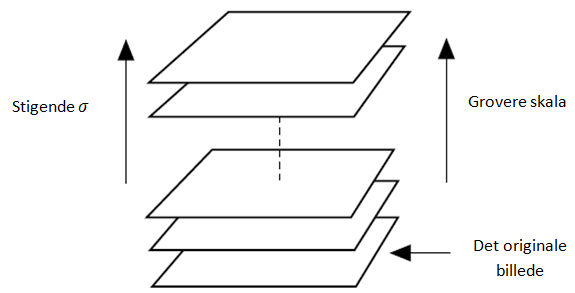
\includegraphics[width=0.55\textwidth]{fig/32.png}
     \vspace{-0.5em}
    \begin{center}    
       \caption{{\footnotesize \textit{En lineær skalarums repræsentation, af et billede. Skalabillederne opstilles som en stak af billeder udsat for stigende grad af slørring}}}
    \label{fig:scalerep}
     \end{center}
     \vspace{-2.5em}
  \end{figure} \noindent
Denne overgang fra finere til grovere strukturer kan opnås ved systematisk at folde billederne med et Gaussisk filter af stigende $\sigma$ værdi, hvor det nederste billede i stakken kan repræsenteres ved biledet $ L(x,y,0) = I(x,y)$ og for $\sigma>0$, defineres et skalabillede $I_\sigma(x,y)$ ved:
\begin{equation}
L(x,y,\sigma) = G(x,y,\sigma)\ast I(x,y)
\label{scalespace1}
\end{equation}
\\
Filteret der bruges til at oprette en skalarumsrepræsentation, skal opfylde følgende egenskaber:
\begin{itemize}
\item{Et lokalt ekstrema må ikke forøges når skala parametren stiger. Dvs. at intensiteten hos et maksima eller minima ikke må respektivt forøges eller formindskes. Dette medfører at nye detaljer ikke må tilføjes, når skalaparametren stiger \cite{lindkth}.}
\item{Hvis hver udglatnings kerne er tilknyttet en skalaparameter, og to kerner foldes med hinanden, ønskes det at den resulterende kerne har en skalaparameter, lig med summen af de foregående skalaparametre \cite{springer}.
\begin{equation}
g(\cdot;\sigma_1) \ast g(\cdot;\sigma_2)=g(\cdot;\sigma_1+\sigma_2)
\label{semi}
\end{equation}
Ovenstående definere at alle skalarums transformationer er af samme familie. En skalarums repræsentation ved en grov skala $\sigma_2$, kan derved udledes ved en repræsentation fra en finere skala:
\begin{equation}
g(\cdot;\sigma_2) = g(\cdot;\sigma_2-\sigma_1)\ast g(;\sigma_1)\text{     hvor     }\sigma_2>\sigma_1
\end{equation}}
\end{itemize}
Der anvendes et Gaussisk filter da den imødekommer begge ovenstående egenskaber. Ved et Gaussisk filter vil strukturer, der eksistere på grovere skalaer være simplificeringer af strukturer fra finere skalaer. Der kan derved ikke opstå nye strukturer ud af ingenting ved anvendelse af det Gaussiske filter. Witkin \cite{witkins} beviste dette i tilfældet for én-dimensionsalle signaler illustreret i figur \ref{scalespace1}, der viser resultatet af at glatte et signal med et Gaussisk filter af stigende $\sigma$ værdi. Det ses tydeligt, hvordan signalets underliggende grovere struktur bliver udtrykt og at finere strukturer undertrykkes.
\begin{figure}[H]
    \centering
    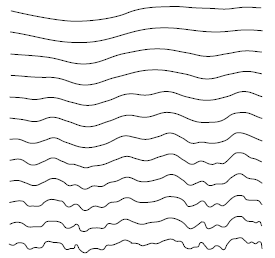
\includegraphics[width=0.45\textwidth]{fig/33.png}
     \vspace{-1em}
    \begin{center}    
       \caption{{\footnotesize \textit{Et én-dimensionalt signal udsat for et Gaussisk filter af gradvist stigende størrelse.}}}
    \label{fig:scalereps}
     \end{center}
     \vspace{-2.5em}
  \end{figure} \noindent
<Måske billede fra lindenscale du ved hvad jeg snakker om Chris>
\subsubsection*{Skala Pyramide}
En udbredt metode, hvorpå skalarummet kan repræsenteres, er ved en \textit{skalapyramide}. Ved en skalapyramide repræsentation oprettes en pyramide af kopier af det undersøgte billede, hvor der for hvert niveau i pyramiden sker en reduktion af billedets størrelse, med en faktor af to. 
Når billedets størrelse skal halveres, er det ikke nok bare at fjerne, hver anden række og hver anden kolonne, da dette vil resultere i store tab af billedets informationer. For at imødekomme dette problem, foldes billedet med et Gaussisk filter, inden billedet reduceres. <Et gaussisk filter anvendes da det flader billedet ud, hvilket formindsker tabet af information>. <Generelt ønskes det at sigma værdien for et Gaussiske filter er fordoblet for hver reduktion af billedet.>
 \begin{figure}[H]
    \centering
    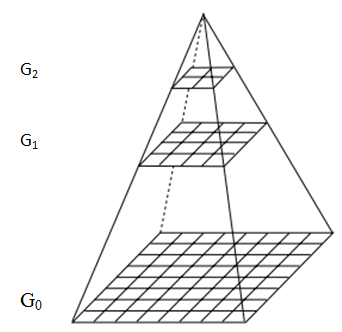
\includegraphics[width=0.40\textwidth]{fig/40.png}
     \vspace{-1em}
    \begin{center}    
       \caption{{\footnotesize \textit{En pyramiderepræsentation af et billede, der reduceres med en faktor af to, for hvert niveau. }}}
    \label{fig:scalerepdiff}
     \end{center}
     \vspace{-2.5em}
  \end{figure} \noindent
Hvis $G_0=I(x,y)$, kan de forskellige niveauer $l$ i skalapyramiden opnås ved:
\begin{equation}
G_l(i,j)=\sum\limits_{m}\sum\limits_{n}w(m,n)G_{l-1}(2i+m,2j+n)
\end{equation}
hvor $w$ er et Gaussisk filter. Fordelene ved en pyramiderepræsentation er at billedernes størrelser reduceres, hvilket reducere antallet af beregninger drastisk.